\documentclass[conference]{IEEEtran}
\usepackage{cite}
\usepackage{amsmath,amssymb,amsfonts}
\usepackage{algorithmic}
\usepackage{graphicx}
\usepackage{textcomp}
\usepackage{xcolor}
\def\BibTeX{{\rm B\kern-.05em{\sc i\kern-.025em b}\kern-.08em
    T\kern-.1667em\lower.7ex\hbox{E}\kern-.125emX}}

\begin{document}

\title{A Survey on Information Managment in Digital Twins Across Industries}
\author{\IEEEauthorblockN{Steven Thompson}
    \IEEEauthorblockA{\textit{Department of Computer Engineering} \\
        \textit{Missouri University of Science And Technology}\\
        Rolla, United States \\
        swth4c@umsystem.edu}
}

\maketitle

\begin{abstract}
    Efficient information management is a challenge that affects every industry attempting to create digital twins, making it one of the primary bottlenecks when adopting this technology. Additionally, each industry defines digital twins differently, resulting in very low interoperability of digital twin architecture across industries. However, despite the varying definitions, the core of digital twins are oftentimes processing large amounts of heterogeneous data. This study examines the degree to which the varying definitions of digital twins effect the information management requirements and methods in digital twin implementations. Furthermore, this study evaluates how well these methods can be adapted to different industries, identifying both open challenges with adapting these methods and future research directions.
\end{abstract}

\begin{IEEEkeywords}
    digital twin, information management
\end{IEEEkeywords}

\section{Introduction}

The concept of a digital twin, an accurate digital representation of a physical object, has recently become feasible due to advancements in enabling technologies. This technological progress has led to an exponential increase in digital twin research over the last decade. The original motivation behind the development of digital twins was to optimize product lifecycle management, primarily in the manufacturing industry, as a means to support the goals of Industry 4.0. However, through ongoing research, a wide range of applications across various industries have been discovered \cite{mihai_digital_2022} \cite{singh_applications_2022} \cite{b_heluany_survey_2023}.
Digital twins rely on a bidirectional flow of information between the physical and virtual spaces, as illustrated in Figure \ref{fig:digital_twin}. Changes in the virtual space lead to changes in the physical space, and vice versa. As a result, the basic architecture of a digital twin can be defined by three key components:
\begin{enumerate}
    \item The physical object or space
    \item A digital representation of the physical space
    \item A communication channel that links these spaces together
\end{enumerate}

One of the most significant challenges in implementing effective, high-fidelity digital twins is information management \cite{xiong_digital_2022} \cite{boyes_digital_2022}. Digital twins often need to collect and process large volumes of heterogeneous data from both physical and digital sources, making data fusion a critical aspect of their operation.
Fusing physical and digital data is essential to leverage their dependencies and create a comprehensive view of the system. However, ensuring data quality can be challenging, as physical data may be incomplete or incorrect due to issues like power outages or faulty sensors. Efficient data storage is another crucial consideration, as data retention policies may require information to be stored for extended periods. Furthermore, depending on the application, high-speed data communication channels may be necessary to enable real-time monitoring and control. Finally, robust data security and governance practices are essential to protect the digital twin and its associated systems. All communication between the physical and virtual spaces must be secure to maintain the integrity and confidentiality of the data.
\begin{figure}[htp]
    \centering
    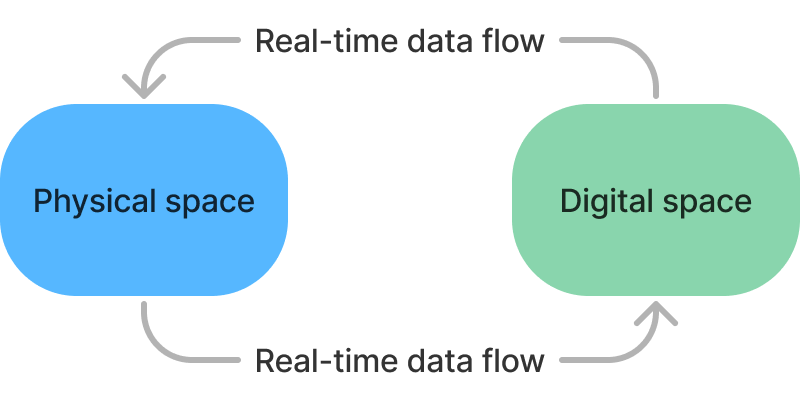
\includegraphics[width=0.4\textwidth]{digital-twin.png}
    \caption{digital twin concept overview}
    \label{fig:digital_twin}
\end{figure}

\subsection{Related Surveys}
This section provides an overview of recent digital twin surveys and their coverage of information management challenges. Table \ref{table:relevant_surveys} summarizes the extent to which each survey addresses data fusion, data quality, data storage, data communication, and data security. The analysis reveals that while some surveys have partially or thoroughly addressed specific information management aspects, a comprehensive survey examining how different industries tackle these challenges has not been conducted. Such a survey could help identify information management practices that can be adapted across industries, facilitating the development of interoperable templates reduce the development time and cost of digital twin implementation.

\checkmark\checkmark - thorough coverage of the topic

\checkmark - partial coverage of the topic

x - no coverage of the topic

\begin{table}[htbp]
    \centering
    \caption{An overview of digital twin surveys since 2022}
    \resizebox{\columnwidth}{!}{%
        \label{table:relevant_surveys}
        \begin{tabular}{|c|c|c|c|c|c|}
            \hline
            reference                      & fusion               & quality              & storage              & communication        & security             \\
            \hline
            \cite{mihai_digital_2022}      & x                    & \checkmark           & x                    & \checkmark\checkmark & \checkmark\checkmark \\
            \hline
            \cite{singh_applications_2022} & x                    & x                    & x                    & x                    & x                    \\
            \hline
            \cite{b_heluany_survey_2023}   & x                    & x                    & \checkmark           & \checkmark           & \checkmark\checkmark \\
            \hline
            \cite{xiong_digital_2022}      & \checkmark\checkmark & \checkmark           & x                    & x                    & x                    \\
            \hline
            \cite{boyes_digital_2022}      & x                    & \checkmark           & \checkmark           & \checkmark           & \checkmark           \\
            \hline
            This survey                    & \checkmark\checkmark & \checkmark\checkmark & \checkmark\checkmark & \checkmark\checkmark & \checkmark\checkmark \\
            \hline
        \end{tabular}%
    }
\end{table}

\subsection{Research Methodology}
This survey attempts to answer the following research questions:

\begin{enumerate}
    \item How do information management requirements change across industries?
    \item What approaches are different industries currently applying to meet these requirements?
    \item How can these methods be adapted across industries?
\end{enumerate}

\subsection{Survey Structure}
The survey categorizes related works based on the following industries: (1) manufacturing, (2) aerospace, (3) automotive, (4) energy, (5) construction, (6) marine, (7) healthcare, and (8) education. For each category, relevant papers have been identified for discussion, and additional references will be included in the full submission.

For category (1), papers \cite{lam_bibliometric_2023} \cite{jyeniskhan_digital_2023} \cite{zhao_research_2023} \cite{chen_data_2023} will be discussed

For category (2), papers \cite{xiong_digital_2022} \cite{hua_leveraging_2023} \cite{diange_research_2022} will be discussed

For category (3), papers \cite{s_design_2023} \cite{xie_digital_2022} \cite{gross_transition_2023} will be discussed

For category (4), papers \cite{gu_digital_2022} \cite{zhifeng_distribution_2023} \cite{nwoke_fpga-based_2023} \cite{qiao_research_2023} will be discussed

For category (5), papers \cite{sabri_designing_2023} \cite{xinying_digital_2023} \cite{furuta_web-based_2023} will be discussed

For category (6), papers \cite{bartolucci_digital_2022} \cite{lv_digital_2023} will be discussed

For category (7), papers \cite{shrivastava_review_2023} \cite{viceconti_position_2024} \cite{pirbhulal_towards_2022} will be discussed

For category (8), papers \cite{tabunshchyk_digital_2023} \cite{fashal_review_2023} will be discussed


\subsection{Contributions}

The primary contributions of this survey are:
\begin{enumerate}
    \item A comprehensive analysis of information management methods employed by industries utilizing digital twin technology, focusing on (1) data fusion, (2) data fidelity, (3) data storage, (4) data communication, and (5) data security and governance.
    \item An evaluation of how these methods can be adapted and applied across industries.
    \item Identification of open challenges and future research directions in the field of information management for digital twins.
\end{enumerate}

To the best of my knowledge, no comprehensive analysis of the aforementioned information management methods for digital twins across different industries currently exists.

\bibliographystyle{IEEEtran}
\bibliography{digital-twin}

\end{document}
